\newcommand{\ket}[1]{\ensuremath{\left|#1\right\rangle}} % Dirac Kets

\newcommand{\qgate}[1]{
    \centerfigureone{
        \begin{tikzpicture}[thick]
        %
        % `operator' will only be used by Hadamard (H) gates here.
        % `phase' is used for controlled phase gates (dots).
        % `surround' is used for the background box.
        \tikzstyle{operator} = [draw,fill=white,minimum size=1.5em] 
        \tikzstyle{phase} = [fill,shape=circle,minimum size=5pt,inner sep=0pt]
        \tikzstyle{surround} = [fill=blue!10,thick,draw=black,rounded corners=2mm]
        %
        % Qubits
        \node at (0,0) (q1) {};
        %
        % Column 1
        \node[operator] (op11) at (1,0) {#1} edge [-] (q1);
        %
        % Column 6
        \node (end1) at (2,0) {} edge [-] (op11);
        %
    \end{tikzpicture}
    }
}

%% two params
%% first param - choose the symbol of controlled gate
%% second param - letter for the gate is any
\newcommand{\qcontrolgate}[2]{
    \centerfiguretwo{
        \begin{tikzpicture}[thick]
            %
            % `operator' will only be used by Hadamard (H) gates here.
            % `phase' is used for controlled phase gates (dots).
            % `surround' is used for the background box.
            % `crossx' is used for the cross.
            % `circlewc' is used for the circle with cross box.
            \tikzstyle{operator} = [draw,fill=white,minimum size=1.5em] 
            \tikzstyle{phase} = [fill,shape=circle,minimum size=5pt,inner sep=0pt]
            \tikzstyle{surround} = [fill=blue!10,thick,draw=black,rounded corners=2mm]
            \tikzstyle{circlewc} = [draw,circle,cross,minimum width=0.3 cm]
            \tikzstyle{cross} = [path picture={ 
                \draw[thick,black](path picture bounding box.north) -- (path picture bounding box.south) (path picture bounding box.west) -- (path picture bounding box.east);
                }]
            \tikzstyle{crossx} = [path picture={ 
                \draw[thick,black,inner sep=0pt]
                (path picture bounding box.south east) -- (path picture bounding box.north west) (path picture bounding box.south west) -- (path picture bounding box.north east);
                }]
            %
            % Qubits
            \node at (0,0) (q1) {};
            \node at (0,-1) (q2) {};
            %
            % Column 1
            \node[phase] (phase11) at (1,0) {} edge [-] (q1);
            \node[#1] (cw12) at (1,-1) {#2} edge [-] (q2);
            \draw[-] (phase11) -- (cw12);
            %
            % Column 2
            \node (end1) at (2,0) {} edge [-] (phase11);
            \node (end2) at (2,-1) {} edge [-] (cw12);
        \end{tikzpicture}
    }
}

\newcommand{\swapgate}{
    \centerfiguretwo{
        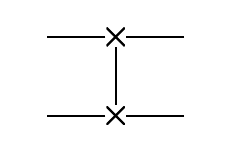
\begin{tikzpicture}[thick]
            %
            % `operator' will only be used by Hadamard (H) gates here.
            % `phase' is used for controlled phase gates (dots).
            % `surround' is used for the background box.
            % `crossx' is used for the cross.
            % `circlewc' is used for the circle with cross box.
            \tikzstyle{operator} = [draw,fill=white,minimum size=1.5em] 
            \tikzstyle{phase} = [fill,shape=circle,minimum size=5pt,inner sep=0pt]
            \tikzstyle{surround} = [fill=blue!10,thick,draw=black,rounded corners=2mm]
            \tikzstyle{circlewc} = [draw,circle,cross,minimum width=0.3 cm]
            \tikzstyle{cross} = [path picture={ 
                \draw[thick,black](path picture bounding box.north) -- (path picture bounding box.south) (path picture bounding box.west) -- (path picture bounding box.east);
                }]
            \tikzstyle{crossx} = [path picture={ 
                \draw[thick,black,inner sep=0pt]
                (path picture bounding box.south east) -- (path picture bounding box.north west) (path picture bounding box.south west) -- (path picture bounding box.north east);
                }]
            %
            % Qubits
            \node at (0,0) (q1) {};
            \node at (0,-1) (q2) {};
            %
            % Column 1
            \node[crossx] (phase11) at (1,0) {} edge [-] (q1);
            \node[crossx] (cw12) at (1,-1) {} edge [-] (q2);
            \draw[-] (phase11) -- (cw12);
            %
            % Column 2
            \node (end1) at (2,0) {} edge [-] (phase11);
            \node (end2) at (2,-1) {} edge [-] (cw12);
        \end{tikzpicture}
    }
}

\newcommand{\toffoligate}{
    \centerfigurethree{
        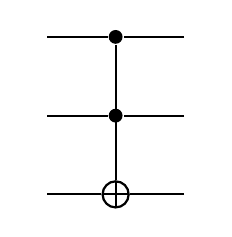
\begin{tikzpicture}[thick]
            %
            % `operator' will only be used by Hadamard (H) gates here.
            % `phase' is used for controlled phase gates (dots).
            % `surround' is used for the background box.
            % `crossx' is used for the cross.
            % `circlewc' is used for the circle with cross box.
            \tikzstyle{operator} = [draw,fill=white,minimum size=1.5em] 
            \tikzstyle{phase} = [fill,shape=circle,minimum size=5pt,inner sep=0pt]
            \tikzstyle{surround} = [fill=blue!10,thick,draw=black,rounded corners=2mm]
            \tikzstyle{circlewc} = [draw,circle,cross,minimum width=0.3 cm]
            \tikzstyle{cross} = [path picture={ 
                \draw[thick,black](path picture bounding box.north) -- (path picture bounding box.south) (path picture bounding box.west) -- (path picture bounding box.east);
                }]
            \tikzstyle{crossx} = [path picture={ 
                \draw[thick,black,inner sep=0pt]
                (path picture bounding box.south east) -- (path picture bounding box.north west) (path picture bounding box.south west) -- (path picture bounding box.north east);
                }]
            %
            % Qubits
            \node at (0,0) (q1) {};
            \node at (0,-1) (q2) {};
            \node at (0,-2) (q3) {};
            %
            % Column 1
            \node[phase] (phase11) at (1,0) {} edge [-] (q1);
            \node[phase] (phase21) at (1,-1) {} edge [-] (q2);
            \node[circlewc] (cw31) at (1,-2) {} edge [-] (q3);
            \draw[-] (phase11) -- (cw31);
            %
            % Column 2
            \node (end1) at (2,0) {} edge [-] (phase11);
            \node (end2) at (2,-1) {} edge [-] (phase21);
            \node (end3) at (2,-2) {} edge [-] (cw31);
        \end{tikzpicture}
    }
}

\newcommand{\measurementgate}{
    \centerfigureone{
        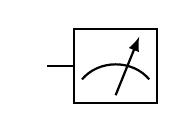
\begin{tikzpicture}[thick]
        %
        % `operator' will only be used by Hadamard (H) gates here.
        % `phase' is used for controlled phase gates (dots).
        % `surround' is used for the background box.
        \tikzstyle{operator} = [draw,fill=white,minimum size=1.5em] 
        \tikzstyle{phase} = [fill,shape=circle,minimum size=5pt,inner sep=0pt]
        \tikzstyle{surround} = [fill=blue!10,thick,draw=black,rounded corners=2mm]
        \tikzset{meter/.append style={draw, inner sep=10, rectangle, font=\vphantom{A}, minimum width=30, line width=.8,
             path picture={\draw[black] ([shift={(.1,.3)}]path picture bounding box.south west) to[bend left=50] ([shift={(-.1,.3)}]path picture bounding box.south east);\draw[black,-latex] ([shift={(0,.1)}]path picture bounding box.south) -- ([shift={(.3,-.1)}]path picture bounding box.north);}}}
        %
        % Qubits
        \node at (0,0) (q1) {};
        %
        % Column 1
        \node[meter] (op11) at (1,0) {} edge [-] (q1);
        %
    \end{tikzpicture}
    }
}

\newcommand{\qubitwire}{
    \centerfigureone{
        \begin{tikzpicture}[thick]
        %
        % `operator' will only be used by Hadamard (H) gates here.
        % `phase' is used for controlled phase gates (dots).
        % `surround' is used for the background box.
        \tikzstyle{operator} = [draw,fill=white,minimum size=1.5em] 
        \tikzstyle{phase} = [fill,shape=circle,minimum size=5pt,inner sep=0pt]
        \tikzstyle{surround} = [fill=blue!10,thick,draw=black,rounded corners=2mm]
        \tikzset{meter/.append style={draw, inner sep=10, rectangle, font=\vphantom{A}, minimum width=30, line width=.8,
             path picture={\draw[black] ([shift={(.1,.3)}]path picture bounding box.south west) to[bend left=50] ([shift={(-.1,.3)}]path picture bounding box.south east);\draw[black,-latex] ([shift={(0,.1)}]path picture bounding box.south) -- ([shift={(.3,-.1)}]path picture bounding box.north);}}}
        %
        % Qubits
        \node at (0,0) (q1) {};
        %
        % Column 1
        \node (op11) at (2,0) {} edge [-] (q1);
        %
        \end{tikzpicture}
    }
}

\newcommand{\classicalwire}{
    \centerfigureone{
        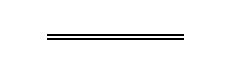
\begin{tikzpicture}[thick]
        %
        % `operator' will only be used by Hadamard (H) gates here.
        % `phase' is used for controlled phase gates (dots).
        % `surround' is used for the background box.
        \tikzstyle{operator} = [draw,fill=white,minimum size=1.5em] 
        \tikzstyle{phase} = [fill,shape=circle,minimum size=5pt,inner sep=0pt]
        \tikzstyle{surround} = [fill=blue!10,thick,draw=black,rounded corners=2mm]
        \tikzset{meter/.append style={draw, inner sep=10, rectangle, font=\vphantom{A}, minimum width=30, line width=.8,
             path picture={\draw[black] ([shift={(.1,.3)}]path picture bounding box.south west) to[bend left=50] ([shift={(-.1,.3)}]path picture bounding box.south east);\draw[black,-latex] ([shift={(0,.1)}]path picture bounding box.south) -- ([shift={(.3,-.1)}]path picture bounding box.north);}}}
        %
        % Qubits
        \node at (0,0) (q1) {};
        %
        % Column 1
        \node (op11) at (2,0) {} edge[double] [-] (q1);
        %
        \end{tikzpicture}
    }
}